\documentclass[twoside]{article}
\usepackage{graphicx}
\usepackage{algorithm}% http://ctan.org/pkg/algorithm
\usepackage{algpseudocode}% http://ctan.org/pkg/algorithmicx
\usepackage{blindtext} % Package to generate dummy text throughout this template 

\usepackage[sc]{mathpazo} % Use the Palatino font
\usepackage[T1]{fontenc} % Use 8-bit encoding that has 256 glyphs
\linespread{1.05} % Line spacing - Palatino needs more space between lines
\usepackage{microtype} % Slightly tweak font spacing for aesthetics

\usepackage[english]{babel} % Language hyphenation and typographical rules

\usepackage[hmarginratio=1:1,top=32mm,columnsep=20pt]{geometry} % Document margins
\usepackage[hang, small,labelfont=bf,up,textfont=it,up]{caption} % Custom captions under/above floats in tables or figures
\usepackage{booktabs} % Horizontal rules in tables

\usepackage{lettrine} % The lettrine is the first enlarged letter at the beginning of the text

\usepackage{enumitem} % Customized lists
\setlist[itemize]{noitemsep} % Make itemize lists more compact

\usepackage{abstract} % Allows abstract customization
\renewcommand{\abstractnamefont}{\normalfont\bfseries} % Set the "Abstract" text to bold
\renewcommand{\abstracttextfont}{\normalfont\small\itshape} % Set the abstract itself to small italic text

\usepackage{titlesec} % Allows customization of titles
\renewcommand\thesection{\Roman{section}} % Roman numerals for the sections
\renewcommand\thesubsection{\roman{subsection}} % roman numerals for subsections
\titleformat{\section}[block]{\large\scshape\centering}{\thesection.}{1em}{} % Change the look of the section titles
\titleformat{\subsection}[block]{\large}{\thesubsection.}{1em}{} % Change the look of the section titles

\usepackage{fancyhdr} % Headers and footers
\pagestyle{fancy} % All pages have headers and footers
\fancyhead{} % Blank out the default header
\fancyfoot{} % Blank out the default footer
\fancyhead[C]{Sudoku validation as a pattern recognition problem $\bullet$ Oct 2019} % Custom header text
\fancyfoot[RO,LE]{\thepage} % Custom footer text

\usepackage{titling} % Customizing the title section

\usepackage{hyperref} % For hyperlinks in the PDF

%----------------------------------------------------------------------------------------
%	TITLE SECTION
%----------------------------------------------------------------------------------------

\setlength{\droptitle}{-4\baselineskip} % Move the title up

\pretitle{\begin{center}\Huge\bfseries} % Article title formatting
\posttitle{\end{center}} % Article title closing formatting
\title{Sudoku validation as a pattern recognition problem} % Article title
\author{%
\textsc{Charu Agarwal} \\[1ex] % Your name
\normalsize Indian Insitute of Technology, Dharwad \\ % Your institution
\normalsize \href{mailto:160010038@iitdh.ac.in}{160010038@iitdh.ac.in} % Your email address
}
\date{\today} % Leave empty to omit a date
\renewcommand{\maketitlehookd}{%
\begin{abstract}
\begin{center}
\noindent This paper is an exploration of using neural networks to understand the constraints of knowledge games. We have considered the problem of checking whether a fully-filled sudoku board configuration is valid or invalid. The goal is to automatically infer the rules of sudoku from examples, without explicitly specifying them. We give an architecture of a model which may be suitable for this problem. While we have achieved good results for most errors, the model is not able to generalize for all cases. We consider some reasons when a problem may not be implicitly solvable by neural networks.
\end{center}
\end{abstract}
}

%----------------------------------------------------------------------------------------

\begin{document}

% Print the title
\maketitle

%----------------------------------------------------------------------------------------
%	ARTICLE CONTENTS
%----------------------------------------------------------------------------------------

\section{Introduction}

\lettrine[nindent=0em,lines=3]{S} udoku is a combinatorial \cite{lawler} number placement puzzle based on logical reasoning \cite{arnoldy}. The objective is to fill a 9x9 grid with digits so that each column, each row, and each of the nine 3x3 subgrids that compose the grid (also called "boxes", "blocks", or "regions") contain all of the digits from 1 to 9. The general sudoku problem is to reach a solution from a partially completed grid \footnote{For a well-posed puzzle there exists a unique solution.}. Figure \ref{fig:sudoku} shows how a typical sudoku puzzle looks like.

Our goal is to train a neural network to understand the constraints of the sudoku. Particularly, given a board configuration, the model should be able to predict whether the configuration is valid or invalid. For the sake of simplicity, we have considered only fully-filled grids.

Now, one may argue the need of neural networks as this problem can be easily solved using an algorithm such as algorithm \ref{algo:algo1}. Similar work has been done in \cite{fizzbuzz}, where the problem of "Fizz Buzz"\footnote{The problem of fizzbuzz is defined as follows: print the numbers from 1 to 100, except that if the number is divisible by 3 print "fizz", if it's divisible by 5 print "buzz", and if it's divisible by 15 print "fizzbuzz".} has been solved using neural networks with fair accuracy, but not reliably. The challenge is not to complicate simple problems by posing them as pattern recognition problems, but to develop a model which can automatically infer the rules of a game, without explicitly stating them. Simple problems can sometimes contain really interesting subtleies.

Sudoku, along with games such as crossword and wordsearch, roughly falls under the category of brain games which is an active area of research. By applying newly developing technologies in the areas of machine learning to understand how computers may be able to create such knowledge games, we hope to solve problems that have otherwise proven to be hard to solve using heuristic algorithms.

\begin{algorithm}
  \caption{Simple algorithm to classify a sudoku as valid or invalid.}\label{algo:algo1}
  \begin{algorithmic}[1]
    \Procedure{isSudokuValid}{$grid$}\Comment{Validates a sudoku}
      \For{\texttt{each row}}     \Comment{Check for duplicate numbers in each row.}
        \For{\texttt{each number $k$ in $1..n$}}
         	\If{k is not in row}
    			\State \textbf{return} $False$
    		\EndIf
      	\EndFor
      \EndFor

      \For{\texttt{each column}}  \Comment{Check for duplicate numbers in each column.}
        \For{\texttt{each number $k$ in $1..n$}}
         	\If{k is not in column}
    			\State \textbf{return} $False$
    		\EndIf
      	\EndFor
      \EndFor

      \For{\texttt{each block}}  \Comment{Check for duplicate numbers in each block.}
        \For{\texttt{each number $k$ in $1..n$}}
         	\If{k is not in block}
    			\State \textbf{return} $False$
    		\EndIf
      	\EndFor
      \EndFor

      \State \textbf{return} $True$    
      \EndProcedure
  \end{algorithmic}
\end{algorithm}

\begin{figure*}
  \centering
  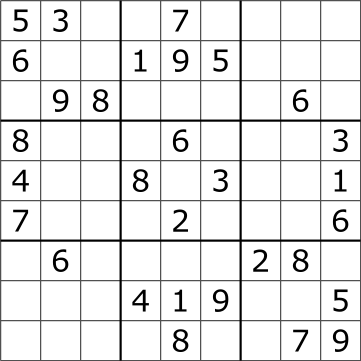
\includegraphics[height=200pt]{typical_sudoku.png}
  \caption{A typical sudoku puzzle.}
  \label{fig:sudoku}
\end{figure*}

\section{The Dataset}
The sudoku puzzles for training have been taken from  \cite{bryan_park}. The data contains 1 million sudoku games and solutions. The solutions are all valid solutions. Hence, for our purpose, we decide to generate invalid sudokus from the valid ones. In the generation of invalid dataset, for each invalid instance, the valid instance was included in the training data. This would make the learning difficult as close samples are in both positive and negative class. 
\\ The valid and invalid sudokus generated together form a dataset of 2 million samples. Depending of the method of generating invalid puzzles, we form three different datasets:

\begin{itemize}
	\item Dataset A: In this dataset, 50\% of the values (on an average) of the sudoku are in error. This has been achieved by shifting the value of some elements by a random integer between 1 - 8.
	\item Datase B: In this dataset, one error has been introduced in the sudoku. This has been achieved by shifting the value of a random element by a random integer between 1 - 8.
	\item Dataset C: In this dataset, errors are introduce such that exactly one constraint (row/column/block) is not satisfied, while the other two constraints are satisfied. This is so that we get a more general distribution of errors. Figure \ref{fig:transformations} gives a schematic diagram of the transformations implemented.
\end{itemize}

\begin{figure*}
  \centering
  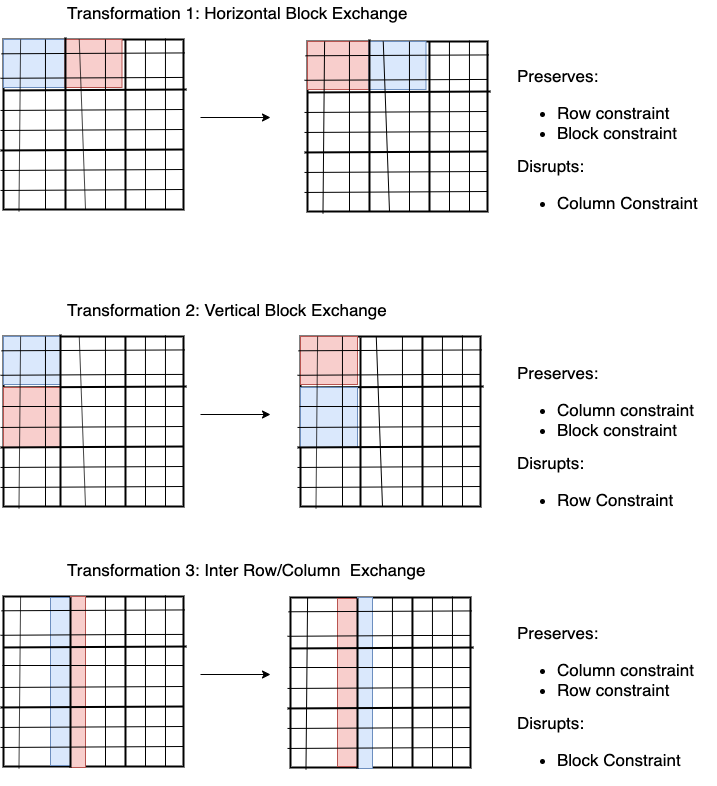
\includegraphics[width=\textwidth]{transformations.png}
  \caption{Transformations to convert a valid sudoku to invalid such that only one constraint is disrupted.}
  \label{fig:transformations}
\end{figure*}

The elements in the grid were standardized onto unit scale and labelled. The dataset after processing is shown in figure \ref{fig:data}.
\begin{figure*}
  \centering
  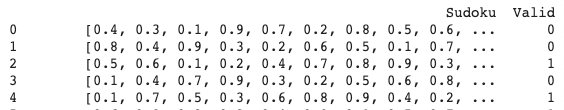
\includegraphics[width=\textwidth]{sample_data.png}
  \caption{Sample data used for training.}
  \label{fig:data}
\end{figure*}

\section{The Architecture}
The performance of a model depends highly on the network topology, the learning law and the activation dynamics. Hence, we have carefully designed our model keeping in mind the advantages and disadvantages of particular neural networks. The architecture of our network is summarized in figure \ref{fig:model}. We have three Convolutional Neural Network layers at the input, which have one filter each:
\begin{itemize}
	\item Row sum layer: This layer consists of one 1x9 filter, with stride 1, to sum up the elements in each row. 
	\item Column sum layer: This layer consists of one 9x1 filter, with stride 1, to sum up the elements in each column.
	\item Block sum layer: This layer consists of one 3x3 filter with stride 3 to sum up the elements in each block.
\end{itemize}
 Convolutional neural network (CNN) is well suited for pattern classification and is designed specifically to recognize two-dimensional shapes with a high degree of invariance to translation, scaling, skewing, and other forms of distortion \cite{haykin}. The salient features of this model are local knowledge (each neuron takes inputs from a local receptive field in the previous layer, thereby forcing it to extract local features) and weight sharing (individual neurons are constrained to share the same weights).
The rationale behind this choice is that if all the filter weights converge to 1, then the model should be able to detect anamolies in the filling (in most cases), as at least one of the filter outputs will not be equal to $4.5$.\footnote{Note that the sum conditions are necessary but not sufficient for a sudoku to be valid. For example, the sequence: 4 4 4 9 5 7 9 2 1 has sum 45.}\\

Next, we have a layer which flattens and concatenates the outputs of the CNNs. The output vector is flattened and concatenated in the form $[x_1, x_2, …, x_{27}]$ where $x_1-x_9$ are the outputs from block sum layer, $x_{10}-x_{18}$ are the outputs from row sum layer and $x_{19}-x_{27}$ are the outputs from the column sum layer.
We add Gaussian Noise with mean 0 and standard deviation 0.01 to increase the spread of the valid class. \footnote{The only example of the valid class is [4.5, 4.5, …, 4.5]}. Finally, the output was fed to a standard two-class classification network: MLP with relu transfer functions, 2 layers of 32 neurons each with Adam for optimization. A multilayer feedforward neural network with backpropagation learning on a finite set of independent and identically distributed samples leads to an asymptotic approximation of the underlying a posteriori class probabilities provided that the size of the training set data is large, and the learning algorithm does not get stuck in a local minimum \cite{hampshire}.\\

\begin{figure*}
  \centering
  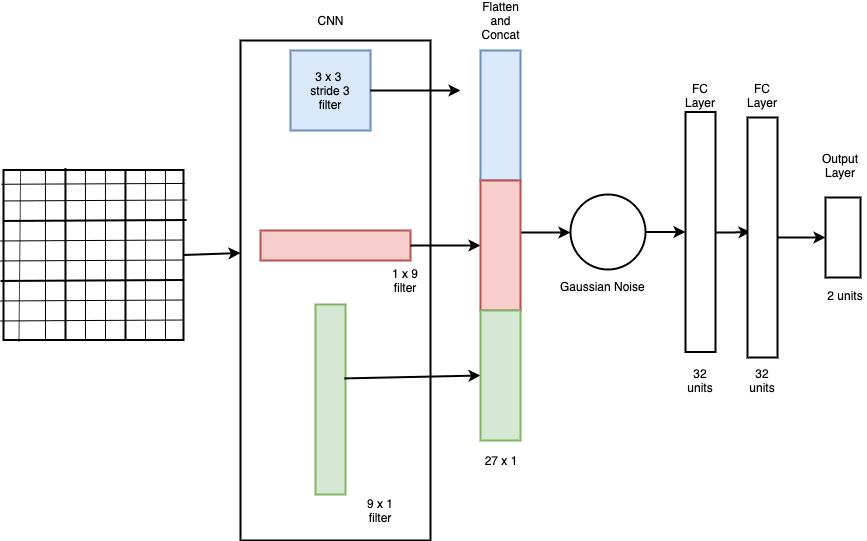
\includegraphics[width=\textwidth]{cnn_fixed_weights.png}
  \caption{An illustration of the architecture of our network for classifying sudokus as valid and invalid.}
  \label{fig:model}
\end{figure*}

%------------------------------------------------

\section{Evaluation Metrics}
We consider five standard metrics for evaluating the model:
\begin{itemize}
	\item Accuracy: Accuracy is the fraction of predictions that are correct. \\
	\begin{equation}
	Accuracy = \frac{TP + TN}{TP + TN + FP + FN}
	\end{equation}
	where TP = True Positives, TN = True Negatives, FP = False Positives, and FN = False Negatives.
	\item Loss: It is a summation of the errors made for each example in training or validation sets.
	\item Precision: Precision is defined as the fraction of postive identifications that are actually correct.
	\begin{equation}
	Precision = \frac{TP}{TP + FP}
	\end{equation}
	\item Recall: Recall is the proportion of actual positives that are identified correctly.
	\begin{equation}
	Recall = \frac{TP}{TP + FN}
	\end{equation}
	\item AUROC: AUROC stands for "Area under the ROC Curve." An ROC curve (receiver operating characteristic curve) is a graph showing the performance of a classification model at all classification thresholds. AUROC can be interpreted as the probability that the model ranks a random positive example more highly than a random negative example. 
\end{itemize}

\section{Results}
First we fixed the weights of each filter to [1, 1, .., 1] and allowed the MLP to learn the weights for classification. This gave us good accuracy $(>96\%)$. Hence, next we unclamped the network and allowed it to learn the filter weights too. Also, we seeded our experiments for reproducible results, and noticed the accuracy of the model varied strongly with the seed value. \\
Table \ref{tab:table1} summarizes the results obtained from the model. While the model achieves excellent accuracy for dataset A and dataset B, it performs fairly well for dataset C. From the precision and recall, we can observe that both dataset A and C result in more false positives, indicating model is more likely to classify a sudoku as valid than invalid. The AUROC is 1 for datasets A and B, indicating that negative samples are ranked strictly below positive samples. For all the datasets, the AUROC is more than 0.5, which means the model performs significantly better than a random classifier.


\begin{table}[h!]
  \begin{center}
    \caption{Results for sudoku classification}
    \label{tab:table1}
    \begin{tabular}{c|c|c|c|c|c}
      \textbf{Dataset} & \textbf{Test Acccuracy} & \textbf{Test Loss} &  \textbf{Precision} &  \textbf{Recall} &  \textbf{AUROC} \\ 
      \hline
      A & 0.99 & 1.86e-05 & 0.99 & 1.00 & 1.00\\
      B & 1 & 6.56e-07& 1.00 & 1.00 & 1.00\\
      C & 0.72 & 0.50 & 0.64 & 0.99 & 0.73 \\
      \hline
    \end{tabular}
  \end{center}
\end{table}
%------------------------------------------------

\section{Discussion}
In this section, we try to understand why the model works for most cases, and more importantly, why it is not able to classify a general problem. To understand why the model is able to classify well for dataset A and dataset B, we decided to look at the filter weights learnt by the model. Figure \ref{fig:filter} shows the filter weights before and after learning. The model has learnt the column sum filter as $c*[1, 1, ..., 1]$ (for some constant c), which is able to detect most errors. We observe that not much learning has occured for the other two filters. This will not work for the general case where the errors may be such that the net sum of errors along a column is zero, although the errors themselves are non zero. \\
On intializing the filter weights with Gaussian Noise with mean 1 and standard deviation 0.01, all the filter weights converge to $c*[1, 1, ..., 1]$ (for some constant c). However, if we increase the variance of the Gaussian Noise to 1, the filter weights are not learnt.
We had considered the possibilty that only one filter weights are being learnt because it is not necessary for the model to learn the other two filters, since one filter is sufficient to detect most errors.\footnote{Part of the reason why dataset C was introduced, since it disrupts only one constraint at a time.} However, this hypothesis was disproved as we tried to train the model with only the block sum filter, but still it was unable to learn the weights.\\
% TODO: Filter weights for dataset C %/
We decided to visualize the datasets using dimensionality reduction techniques: Principal Component Analysis (PCA) and t-Distributed Stochastic Neighbouring Entities (t-SNE). Figures \ref{fig:plot1}, \ref{fig:plot2} and \ref{fig:plot3} show the plots for the datasets. We found that while the valid and invalid classes of dataset A are well-separated, classes of dataset B and C are not easily separable. This may suggest why the model is not able to generalize, since the data itself is inherently not separable into two classes. Overall, t-SNE is able to better cluster the examples into the two classes as compared to PCA.
\begin{figure*}
  \centering
  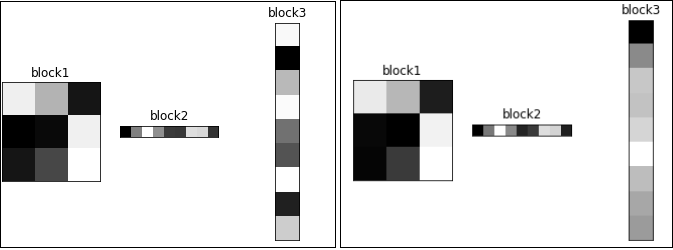
\includegraphics[width=\textwidth]{filters.png}
  \caption{Weights before (left) and after (right) learning. Most of the learning appears to happen in the column sum filter where the weights are all 1.4*. Hence, we can say this filter has understood the constraints as it is assigning almost equal weights to each element. This can explain the good performance of the model. (For most errors, the column filter should be able to detect errors This will not work well for multiple errors where the net sum is 0 within same column.)}
  \label{fig:filter}
\end{figure*}

\begin{figure*}
  \centering
  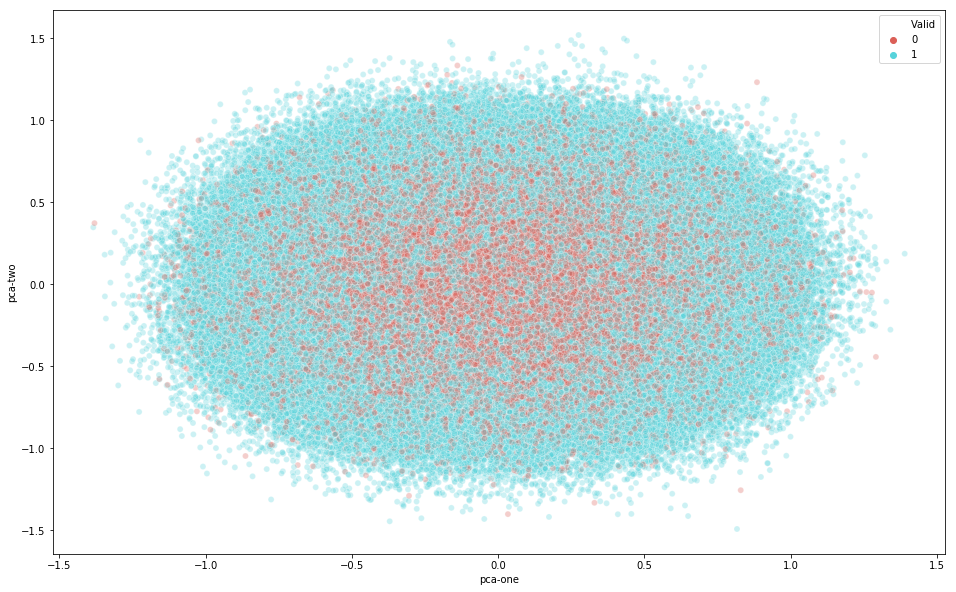
\includegraphics[width=200pt]{sudoku_pca_50error.png}
  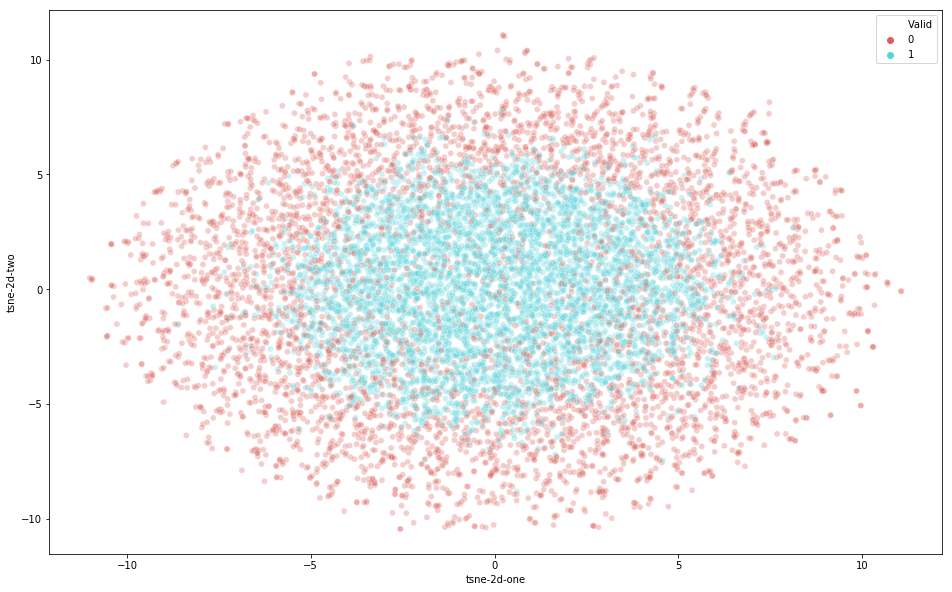
\includegraphics[width=200pt]{sudoku_tsne_50error.png}
  \caption{Visualization of Dataset A (puzzles when 50\% errors are introduced (on an average) in invalid sudokus): PCA (left) vs t-SNE (right)}
  \label{fig:plot1}
\end{figure*}

\begin{figure*}
  \centering
  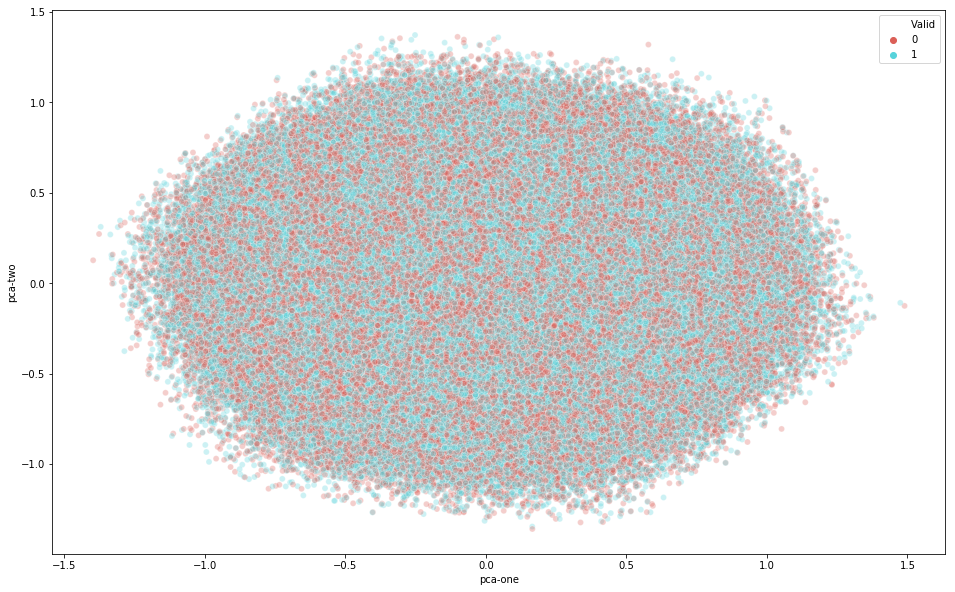
\includegraphics[width=200pt]{sudoku_pca_1error.png}
  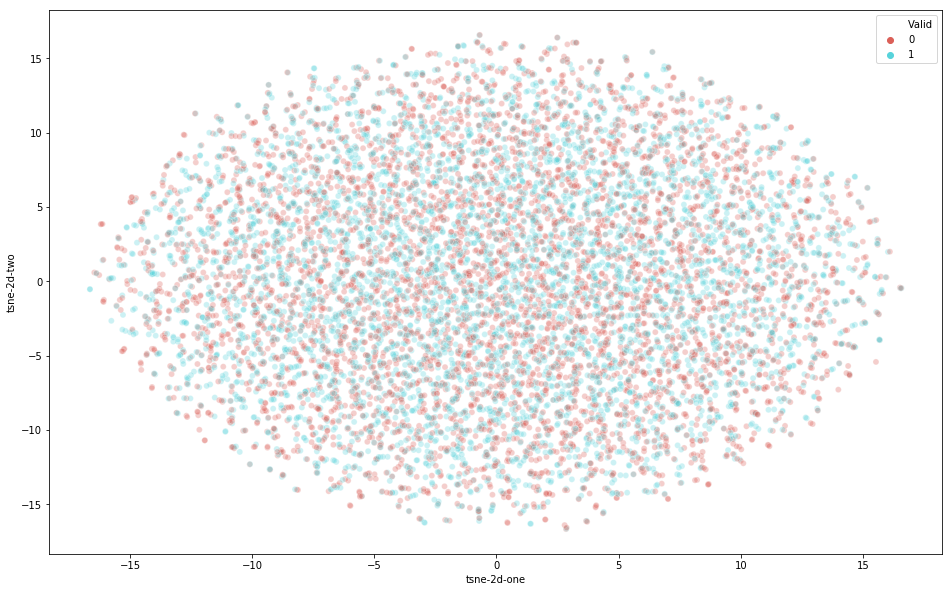
\includegraphics[width=200pt]{sudoku_tsne_1error.png}
  \caption{Visualization of Dataset B (puzzles when 1 error is introduced in invalid sudokus): PCA (left) vs t-SNE (right)}
  \label{fig:plot2}
\end{figure*}

\begin{figure*}
  \centering
  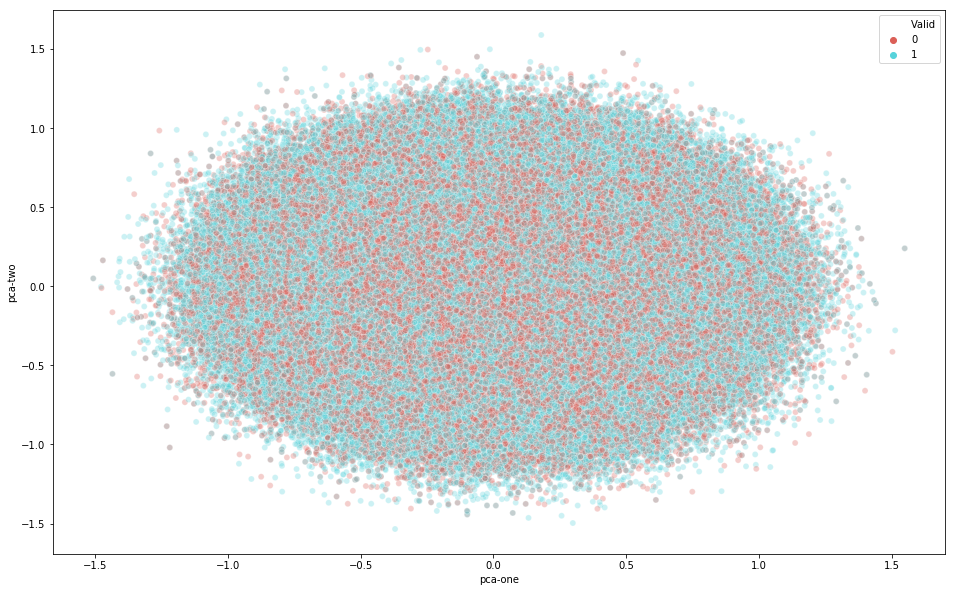
\includegraphics[width=200pt]{sudoku_pca_terror.png}
  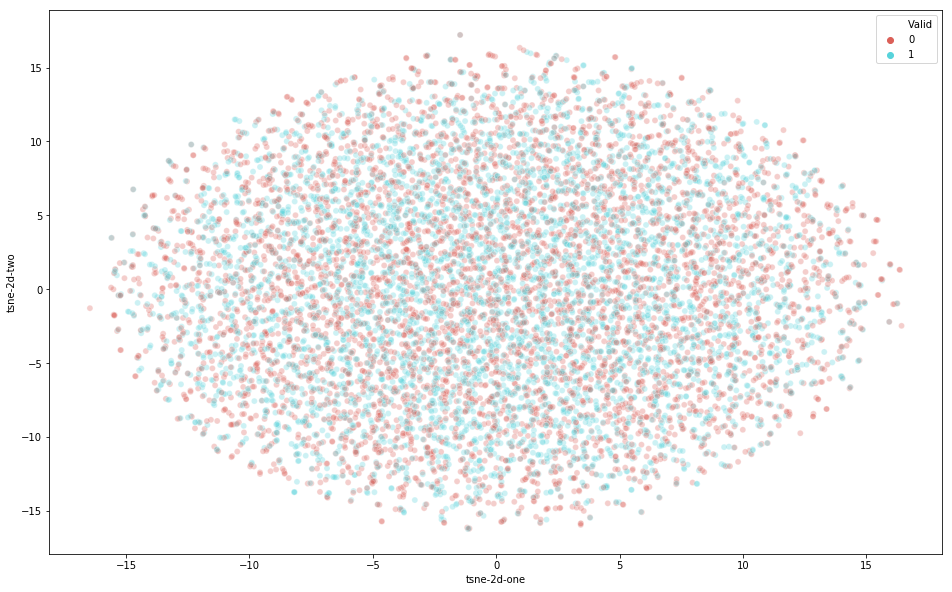
\includegraphics[width=200pt]{sudoku_tsne_terror.png}
  \caption{Visualization of Dataset C (puzzles with one constraint disrupted in invalid sudokus): PCA (left) vs t-SNE (right)}
  \label{fig:plot3}
\end{figure*}

\section{Conclusions}
We considered the idea of modelling the task of validating a completely filled sudoku board configuration as a pattern recognition problem. That is, we wanted to see that given a lot of examples from the valid and invalid classes, can we train a neural network to learn the constraints of sudoku. We proposed a CNN-MLP based model architecture and we observed that while the model is able to classify most samples as valid or invalid correctly, it has only partially learnt the constraints. The good accuracy is attributed to the learning of the column sum filter weights, which allows the model to sum up the elements in each column and detect most forms of discrepancies.\\

We conclude that while we have partially solved the problem of sudoku classification, solving the full problem may require a different model architecture altogether. Observing the data, it seems difficult to model this problem as a pattern recognition problem since the distribution of the valid and invalid class are not well-separated. Our model was quite tailored for the 9x9 sudoku puzzles, but shall not be able to generalize for sudokus of different sizes. But all is not lost, since this might be a small step for sudoku classification, but a significant step for understanding knowledge games. Modeling the problem of learning of the constraints of knowledge games as a pattern recognition problem is a powerful idea, since now we do not need to tell the machine the rules of the games.
\section{Acknowledgements}
This study is the result of many fruitful discussions with Prof. Sudheendra Hangal and Prof. Prabuchandran KJ, who have been the advisors of the project. The author would also like to thank Dept. of Computer Science, IIT Dharwad, for providing the oppurtunity to pursue this problem. This project has been a great learning experience on machine learning problems and has introduced the author to many techniques to design, analyze and debug neural networks.
%----------------------------------------------------------------------------------------
%	REFERENCE LIST
%----------------------------------------------------------------------------------------

\begin{thebibliography}{99} % Bibliography - this is intentionally simple in this template

\bibitem [Park, 2016]{bryan_park}
Kyubyong Park (2016).
\newblock 1 million Sudoku games, Version 3. 
\newblock Retrieved October 6, 2019 from {\em https://www.kaggle.com/bryanpark/sudoku}.

\bibitem [Grus, 2016]{fizzbuzz}
Joel Grus (2016).
\newblock Fizz Buzz in Tensor Flow.
\newblock {\em https://joelgrus.com/2016/05/23/fizz-buzz-in-tensorflow/}.

\bibitem [Arnoldy]{arnoldy}
Ben Arnoldy.
\newblock Sudoku Strategies
\newblock {\em The Christian Science Monitor}.

\bibitem [Lawler, 1985]{lawler}
E. L. Lawler (1985).
\newblock   The Traveling Salesman Problem: A Guided Tour of Combinatorial Optimization.
\newblock {\em West Sussex: John Wiley \& Sons. ISBN 0-471-90413-9}

\bibitem [Haykin, 2009]{haykin}
 S. S. Haykin (2009).
\newblock   Neural networks and learning machines/Simon Haykin.
\newblock {\em New York: Prentice Hall}

\bibitem [Hampshire and Pearlmutter, 1990]{hampshire}
J. B. Hampshire, and B. Pearlmutter (1990).
\newblock   Equivalence proofs for multilayer perceptron classifiers and the Bayesian discriminant function.
\newblock {\em  E InD. S. Touretzky, JL Elman, TJ Sejnowski, and GE Hinton, editors. Proceedings of the 1990 Connectionist Models Summer School. Morgan Kaufmann, San Mateo, CA.}
\end{thebibliography}

%----------------------------------------------------------------------------------------

\end{document}
